\section{问题四的模型建立与求解}

\subsection{求解思路}

问题四在问题二、三的基础上进一步引入\textbf{实时波动电价}。
此时，每天制定购电计划时，不仅未来负载和光伏未知，未来电价也不能提前获得。
若仍按固定电价安排储能，可能在并不便宜的时段提前充电，或在真正的高价时段到来前过早放电。

因此，我们保留前面已经建立的供需预测、误差准备和储能调度模型，只增加一层\textbf{电价预测}，再利用预测价格重新优化购电。

问题四包含两种运行方式：

\begin{itemize}
    \item \textbf{问题四-2：}每天0:00确定当天订单，日内不能修改；
    \item \textbf{问题四-3：}0:00制定原计划，6:00、12:00和18:00可根据新信息调整未执行订单。
\end{itemize}

由于两种情况下能够获得的信息不同，我们分别采用\textbf{提升树预测零点电价}和\textbf{岭回归更新日内电价}。


\subsection{波动电价预测}

历史数据表明，电价具有较稳定的日内轮廓和周重复特征，但同一时刻在不同日期仍有明显波动。为描述这些变化，价格预测同时使用附件1的日内参考电价、过去四周同星期位置的价格中位数、最近七天同刻中位数和上周同刻价格，并加入预测净负荷、星期位置、年内位置及预测提前时间等信息。

日内分支还利用当天已经发生的价格修正后续判断：以实际价格相对历史同刻基线的偏差描述当天整体偏高或偏低的程度，并利用最近一个区间的偏差反映短时变化。净负荷采用当前能够得到的负载与光伏预测之差，不使用未来实际供需。上述信息构成价格模型的特征向量$\mathbf{x}$。

\subsubsection*{（1）问题四-2：提升树价格预测}

每天0:00尚未获得当天实际价格，因此主要依靠历史价格和供需背景预测。
考虑到这些因素与电价之间可能存在非线性关系，我们采用直方图梯度提升树，其形式为

\begin{equation}
\hat{p}
=
F_0(\mathbf{x})
+
\gamma
\sum_{m=1}^{M}
h_m(\mathbf{x}),
\end{equation}

其中，$M=100$，学习率$\gamma=0.05$，最终每棵树最多包含31个叶节点，每个叶节点至少包含50个训练样本。叶节点数控制模型划分不同价格情形的精细程度；限制每个叶节点的样本量，则避免仅依据少数记录作出过细划分。

\subsubsection*{（2）问题四-3：岭回归价格预测}

在6:00、12:00和18:00，可以利用当天已经发生的实际价格更新后续判断。历史同刻价格、近期价格及当天价格偏差之间具有较强相关性，直接回归可能依靠较大的正负系数相互抵消，使预测对小幅变化过于敏感。为限制这种波动，先按当前训练集的均值和标准差将各特征标准化为$\mathbf{z}_i$，再采用岭回归：

\begin{equation}
\min_{\beta_0,\boldsymbol{\beta}}
\sum_i
\left(
p_i-\beta_0-\mathbf{z}_i^{\mathrm T}\boldsymbol{\beta}
\right)^2
+
\lambda
\sum_j\beta_j^2,
\qquad
\lambda=10.
\end{equation}

目标函数中的第一项衡量价格拟合误差，第二项限制回归系数的大小，截距$\beta_0$不受惩罚。各系数由历史数据拟合，可以为负，也不要求和为1。正则参数$\lambda=10$采用候选比较阶段的固定设置，不将后续残差模型的检验结果作为它的选取依据。为使预测价格保持为正，提升树和岭回归的输出均取不低于0.001元/kWh。

价格模型每7天重新训练一次，使用此前56天内已经兑现的历史样本，历史不足时使用已有记录。构造样本时按原决策时点还原特征，避免将后来才知道的价格和供需写入历史输入。日内各时点更新的是模型输入和预测结果，而不是每天重新训练四次模型。


\subsection{波动电价下的购电模型}

\subsubsection*{（1）问题四-2}

问题四-2直接沿用问题二中的负载、光伏预测、误差准备和储能约束，仅将固定电价替换为0:00预测得到的波动电价。

目标函数为

\begin{equation}
\min J_{4-2}
=
\sum_{t\in T_0}
\hat{p}_{t|0}q_t
-
\nu S_T,
\end{equation}

其中，$q_t$为普通购电量，$S_T$为规划末端储电量。

规划仍延伸至次日24:00，以避免模型在当天末尾过早放空电池，但只固定当天订单。
实际运行中，若普通购电和储能仍无法满足负载，则剩余缺口按照该时段\textbf{实际电价的5倍}进行紧急购电。

\subsubsection*{（2）问题四-3}

问题四-3沿用问题三中的滚动调整模型。设零点原计划为$q_t^0$，当前调整后的订单为$q_t$，则滚动优化目标为

\begin{equation}
\min J_{4-3}
=
\sum_{t\in T_r}
\hat{p}_{t|r}
\left(q_t+5e_t\right)
+
\frac{1}{2}
\sum_{t\in D_r}
\hat{p}_{t|r}
\left|q_t-q_t^0\right|
-
\nu S_T,
\end{equation}

其中，$e_t$为预计紧急购电量，$D_r$表示当前时刻尚未执行的当天时段。

已经执行的订单不再修改；同一时段经过多次调整时，只按照最终订单与零点原计划之间的净变化结算。
预测价格只用于制定购电和储能安排。实际运行结束后，普通购电费、调整费和紧急购电费均按对应供电时段的实际价格结算；未被负载或电池接收的普通订单仍需付款。期末库存的参考价值不作为收入从实际费用中扣除。

供需平衡、储电递推、$1200$--$10800\ \mathrm{kWh}$容量限制、$5000\ \mathrm{kW}$充放电功率限制以及$90\%$充放电效率均沿用问题二、三，不再重复列写。


\subsection{模型求解与方案选择}

给定预测电价后，两条分支均转化为线性规划，并采用HiGHS求解。正式统计范围为2025年2月1日至12月31日，共334天。所有价格候选统一从1月份共同启动过程得到的8592.69 kWh内部储电量开始，在各自分支内保持供需预测、设备参数和实际供电规则一致，以比较价格预测方法对调度费用的影响。

三种价格预测方法的比较结果如表所示。

\begin{table}[H]
    \centering
    \caption{波动电价下不同价格预测模型的比较}
    \small
    \begin{tabular}{ccccc}
        \hline
        分支 & 价格模型 & 价格MAE/(元/kWh) & 总费用/万元 & 紧急购电量/kWh \\
        \hline
        问题四-2 & 历史同刻中位数 & 0.04984 & 1427.22 & 97728.89 \\
        问题四-2 & 岭回归 & 0.04472 & 1426.64 & 99205.19 \\
        问题四-2 & 提升树 & \textbf{0.03884} & \textbf{1425.52} & 98725.98 \\
        \hline
        问题四-3 & 历史同刻中位数 & 0.04676 & 1383.78 & 40144.52 \\
        问题四-3 & 岭回归 & 0.04442 & 1382.29 & \textbf{38733.80} \\
        问题四-3 & 提升树 & \textbf{0.03834} & \textbf{1382.06} & 40116.12 \\
        \hline
    \end{tabular}
\end{table}

表中的提升树采用初始15叶设置。问题四-2中，该方案同时取得最低价格预测误差和最低费用，说明历史因素之间的非线性组合有助于零点价格判断。进一步将每棵树的最大叶节点数由15增加至31后，总费用再减少6605.53元，因此最终采用31叶版本。后文最终费用表对应这一深化后的方案，与候选比较表中的15叶结果有所区别。

问题四-3中，提升树虽然比岭回归少花2273.23元，但仅占总费用约$0.016\%$，同时紧急购电量更多、发生紧急购电的日期也更多。因此，最终选择结构更清楚、紧急购电较少的岭回归方案。


\subsection{最终结果与分析}

两种最终方案的全年结果如下。

\begin{table}[H]
    \centering
    \caption{问题四两种最终方案的全年费用结果}
    \begin{tabular}{lrr}
        \hline
        指标 & 问题四-2 & 问题四-3 \\
        \hline
        普通购电费/元 & 13613522.32 & 13327163.05 \\
        调整费/元 & 0.00 & 268515.82 \\
        紧急购电费/元 & 635048.55 & 227222.48 \\
        \textbf{总费用/元} & \textbf{14248570.87} & \textbf{13822901.35} \\
        紧急购电量/kWh & 98756.33 & 38733.80 \\
        期末内部储电量/kWh & 8692.34 & 7918.81 \\
        \hline
    \end{tabular}
\end{table}

允许日内调整后，虽然增加了约26.85万元的调整费用，但普通购电和紧急购电费用下降更多。因此，问题四-3相较问题四-2共减少费用

\begin{equation}
425669.52\ \text{元},
\end{equation}

约下降

\begin{equation}
2.99\%.
\end{equation}

需要指出的是，这一差值同时包含供需信息更新、价格更新和订单调整等多方面作用，不能全部解释为日内价格更新带来的收益。

为比较两种决策方式在具体日期的运行差异，表~\ref{tab:q4_specified_results}列出题目指定日期的普通订单、紧急购电、日末库存和全天费用。其中，普通订单表示最终需要结算的电量，不等于全部被负载或储能实际接收的电量。

\begin{table}[H]
\centering
\caption{问题四指定日期的购电与储电结果}
\label{tab:q4_specified_results}
\small
\begin{tabular}{llrrrr}
\toprule
分支 & 日期 & 普通订单/kWh & 紧急购电/kWh & 日末库存/kWh & 费用/元 \\
\midrule
问题四-2 & 3月20日  & 62329.63 & 329.13 & 1376.30  & 41909.16 \\
         & 6月21日  & 42375.21 & 0.00   & 10380.22 & 20358.11 \\
         & 9月23日  & 68066.93 & 10.23  & 2592.35  & 44700.97 \\
         & 12月21日 & 94612.77 & 0.00   & 9798.14  & 71357.71 \\
\midrule
问题四-3 & 3月20日  & 61795.52 & 93.27  & 1311.14  & 40921.66 \\
         & 6月21日  & 42176.92 & 14.64  & 10800.00 & 20204.97 \\
         & 9月23日  & 67751.81 & 11.32  & 3463.77  & 45250.33 \\
         & 12月21日 & 93283.52 & 20.53  & 8131.62  & 71876.82 \\
\bottomrule
\end{tabular}
\end{table}

允许日内调整并不保证每个日期的费用都更低。例如，问题四-3在3月20日和6月21日的费用较低，在9月23日和12月21日却较高。两种策略也形成了不同的日末库存，并将差异传递至下一天。因此，指定日期用于解释运行差别，整体优劣仍需结合连续统计期的总费用判断。


\subsection{模型检验}

首先，对保存的订单、供需数据和储电轨迹重新逐段计算。共检查865728个10分钟运行区间，储电递推和全年费用的复算误差均处于浮点计算误差范围内，说明求解结果满足所建立的模型约束。

其次，对价格模型和日内更新机制进行进一步检验，结果如图所示。

\begin{figure}[H]
    \centering
    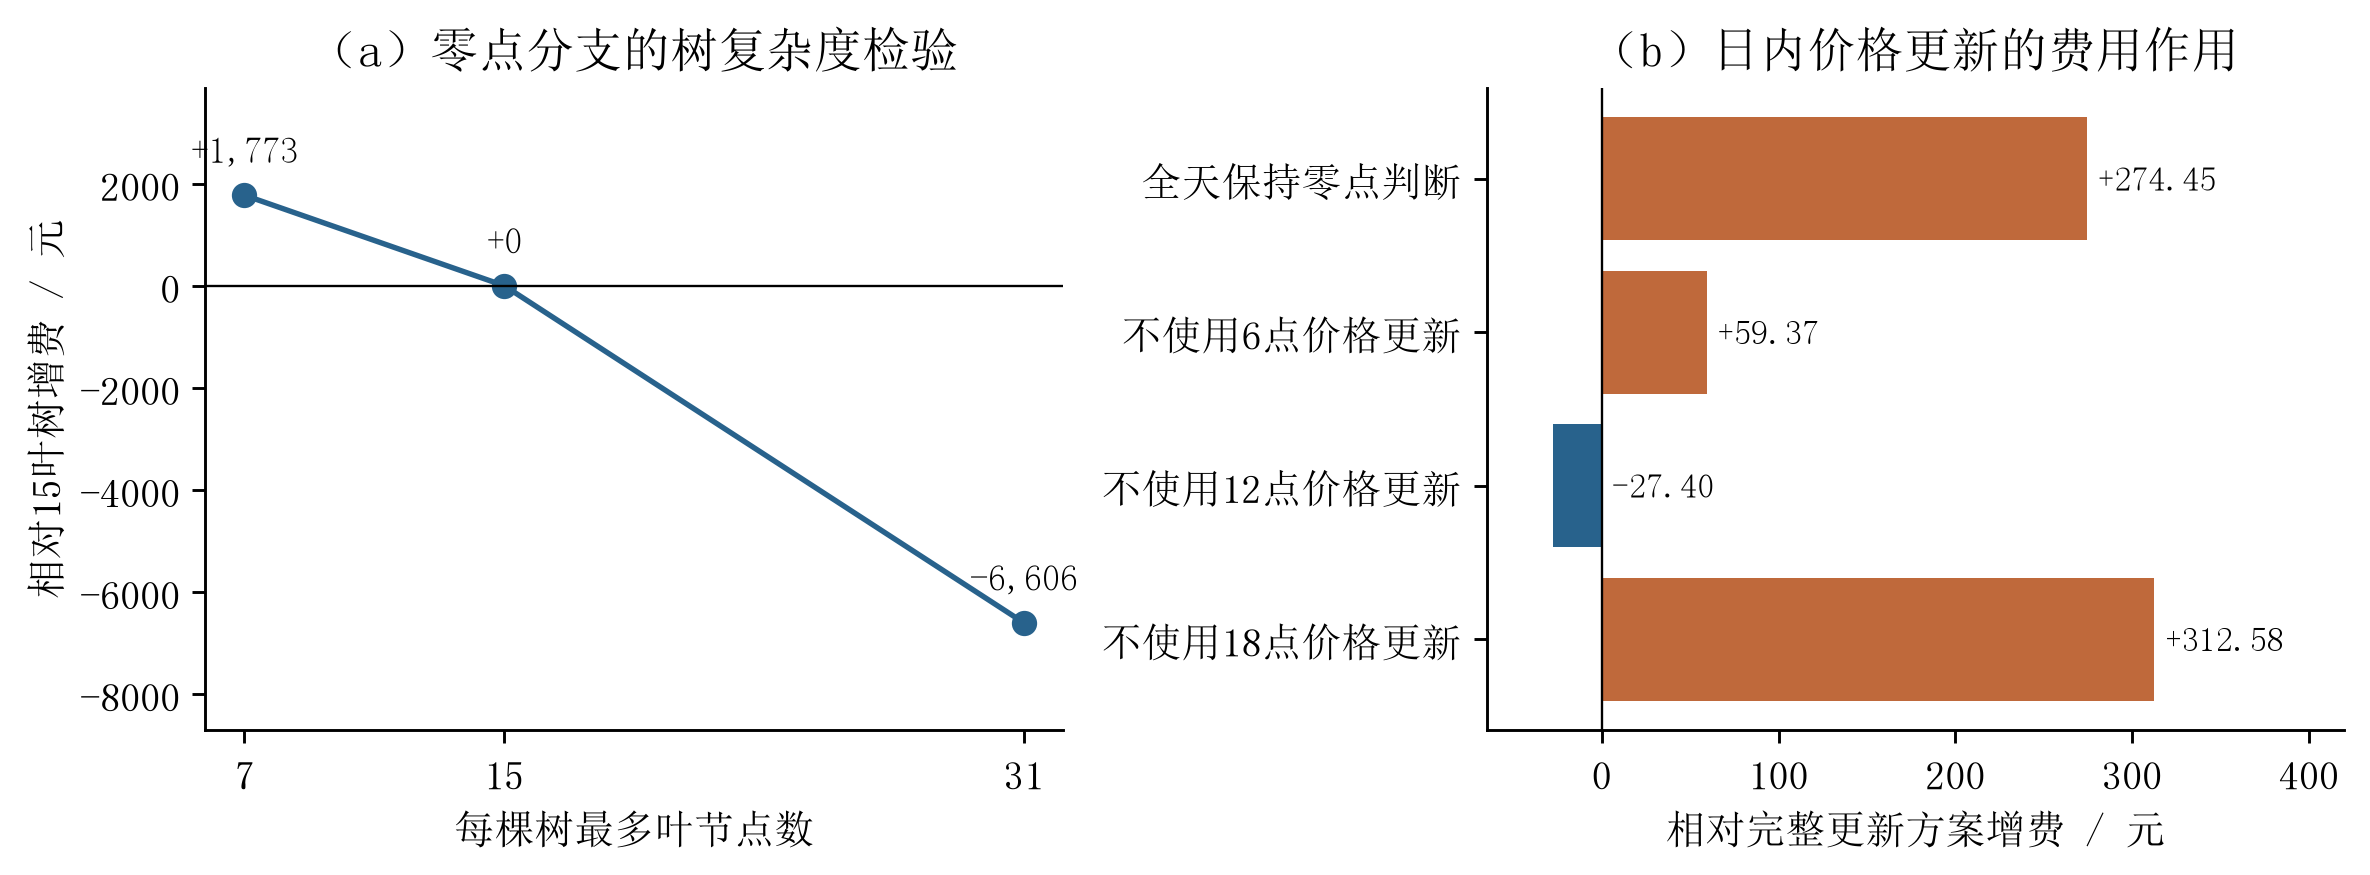
\includegraphics[width=0.95\textwidth]{fig/q4.png}
    \caption{树复杂度与日内价格更新的费用检验}
    \label{fig:q4_model_test}
\end{figure}

\subsubsection*{（1）提升树复杂度检验}

由图\ref{fig:q4_model_test}(a)可见，以15叶模型为基准：

\begin{itemize}
    \item 7叶模型全年费用增加约1773元；
    \item 31叶模型全年费用减少约6606元。
\end{itemize}

因此，在本题比较的三种复杂度下，31叶模型的全年费用最低。不过，该模型仍有部分日期和月份费用高于15叶模型，因此只能说明其在\textbf{本年度总体费用指标下表现更好}。
为排除通过少留期末电量降低费用的影响，进一步按实际价格的第5、第50和第95百分位，对期末最低库存以上的可放电量分别估值。计入剩余电量价值后，31叶方案仍比15叶方案节省5890.24--6423.72元，说明其费用优势并非仅来自期末库存差异。

对于日内分支，还尝试了先确定历史价格基线、再用岭回归预测价格偏差的方式，但所测三档正则强度均未降低费用，因此保留直接预测价格的完整岭回归。

\subsubsection*{（2）日内价格更新检验}

图\ref{fig:q4_model_test}(b)进一步比较不同价格更新方式。以完整的0:00、6:00、12:00和18:00更新方案为基准：

\begin{itemize}
    \item 全天保持零点价格判断，费用增加274.45元；
    \item 不使用6:00价格更新，费用增加59.37元；
    \item 不使用12:00价格更新，费用反而减少27.40元；
    \item 不使用18:00价格更新，费用增加312.58元。
\end{itemize}

结果表明，\textbf{日内价格信息总体具有价值，但并不是每一次更新都一定能够降低费用}。这是因为一次价格更新不仅会改变当前订单，还会改变之后的储电状态，各次更新之间存在相互影响，因此不能将各次费用差简单相加。
在实际价格最高的5\%时段内，问题四-2和问题四-3仍分别发生46086.96 kWh和14665.07 kWh紧急购电。由此可见，储能虽能转移电量，但容量、剩余库存和放电功率仍会限制其缓冲能力，不能完全消除高价与供需偏差叠加时的补购风险。

综上，在波动电价条件下，应先根据当前可获得的历史价格和运行信息预测未来电价，再结合供需预测与储能状态进行统一优化。问题四-2最终采用\textbf{滚动提升树--零点线性规划模型}；问题四-3最终采用\textbf{滚动岭回归--日内调整线性规划模型}。
